\documentclass[12pt,a4paper]{article}

% ===========================================================================
% INFORME DE LABORATORIO N.º 07 - ALGORITMOS AVANZADOS (UNSAAC, 2026-II)
% Tema: Primalidad, grupos y algoritmos probabilísticos
% Formato: Estándar APA 7 / Tipografía Times / Tablas Booktabs / Listings
% Compatible con Overleaf y compilación local con pdflatex
% ===========================================================================

% --- Paquetes de codificación e idioma ---
\usepackage[utf8]{inputenc}
\usepackage[T1]{fontenc}
\usepackage[spanish,es-tabla]{babel}

% --- Geometría y márgenes según pautas APA 7 (1 pulgada / 2.54 cm) ---
\usepackage{geometry}
\geometry{left=2.54cm, right=2.54cm, top=2.54cm, bottom=2.54cm, headheight=15pt}

% --- Tipografía clásica APA ---
\usepackage{mathptmx} % Fuente Times New Roman compatible
\usepackage{setspace}
\onehalfspacing       % Interlineado 1.5 para lectura técnica

% --- Matemáticas y símbolos ---
\usepackage{amsmath, amssymb, amsfonts}

% --- Tablas profesionales (sin líneas verticales según APA 7) ---
\usepackage{booktabs}
\usepackage{array}
\usepackage{tabularx}
\usepackage{multirow}

% --- Figuras y gráficos ---
\usepackage{graphicx}
\usepackage{float}
\usepackage{caption}
\usepackage{subcaption}
\graphicspath{{./}{figuras/}{./figuras/}}

% --- Colores y resaltado de sintaxis para código ---
\usepackage{xcolor}
\definecolor{codegreen}{rgb}{0.13,0.55,0.13}
\definecolor{codegray}{rgb}{0.45,0.45,0.45}
\definecolor{codepurple}{rgb}{0.55,0.0,0.55}
\definecolor{codeblue}{rgb}{0.0,0.2,0.7}
\definecolor{backcolour}{rgb}{0.98,0.98,0.98}
\definecolor{rulecolor}{rgb}{0.85,0.85,0.85}

\usepackage{listings}
\lstdefinestyle{pythonstyle}{
    backgroundcolor=\color{backcolour},
    commentstyle=\color{codegreen}\itshape,
    keywordstyle=\color{codeblue}\bfseries,
    numberstyle=\tiny\color{codegray},
    stringstyle=\color{codepurple},
    basicstyle=\ttfamily\scriptsize,
    breakatwhitespace=false,
    breaklines=true,
    captionpos=b,
    keepspaces=true,
    numbers=left,
    numbersep=4pt,
    showspaces=false,
    showstringspaces=false,
    showtabs=false,
    tabsize=4,
    frame=single,
    rulecolor=\color{rulecolor},
    aboveskip=4pt,
    belowskip=4pt,
    lineskip=-0.8pt,
    literate={á}{{\'a}}1 {é}{{\'e}}1 {í}{{\'i}}1 {ó}{{\'o}}1 {ú}{{\'u}}1
             {ñ}{{\~n}}1 {Á}{{\'A}}1 {É}{{\'E}}1 {Í}{{\'I}}1 {Ó}{{\'O}}1 {Ú}{{\'U}}1 {Ñ}{{\~N}}1
             {≤}{{$\le$}}1 {≥}{{$\ge$}}1 {≠}{{$\neq$}}1
             {≈}{{$\approx$}}1 {∈}{{$\in$}}1 {×}{{$\times$}}1
             {Ω}{{$\Omega$}}1 {→}{{$\to$}}1 {←}{{$\leftarrow$}}1 {≡}{{$\equiv$}}1
             {·}{{$\cdot$}}1 {º}{{$^\circ$}}1 {µ}{{$\mu$}}1 {—}{{---}}1 {…}{{\dots}}1
             {₀}{{$_0$}}1 {₁}{{$_1$}}1 {−}{{-}}1
}

\definecolor{terminalbg}{rgb}{0.96,0.97,0.99}
\definecolor{terminalborder}{rgb}{0.78,0.82,0.88}
\definecolor{terminaltext}{rgb}{0.12,0.18,0.28}

\lstdefinestyle{consolestyle}{
    backgroundcolor=\color{terminalbg},
    basicstyle=\ttfamily\scriptsize\color{terminaltext},
    breaklines=true,
    frame=single,
    rulecolor=\color{terminalborder},
    numbers=none,
    keepspaces=true,
    captionpos=b,
    aboveskip=4pt,
    belowskip=4pt,
    lineskip=-0.8pt,
    literate={á}{{\'a}}1 {é}{{\'e}}1 {í}{{\'i}}1 {ó}{{\'o}}1 {ú}{{\'u}}1
             {ñ}{{\~n}}1 {Á}{{\'A}}1 {É}{{\'E}}1 {Í}{{\'I}}1 {Ó}{{\'O}}1 {Ú}{{\'U}}1 {Ñ}{{\~N}}1
             {≤}{{$\le$}}1 {≥}{{$\ge$}}1 {≠}{{$\neq$}}1
             {≈}{{$\approx$}}1 {∈}{{$\in$}}1 {×}{{$\times$}}1
             {Ω}{{$\Omega$}}1 {→}{{$\to$}}1 {←}{{$\leftarrow$}}1 {≡}{{$\equiv$}}1
             {·}{{$\cdot$}}1 {º}{{$^\circ$}}1 {µ}{{$\mu$}}1 {—}{{---}}1 {…}{{\dots}}1
             {₀}{{$_0$}}1 {₁}{{$_1$}}1 {−}{{-}}1
}
\lstset{style=pythonstyle}

% --- Encabezados y numeración ---
\usepackage{fancyhdr}
\pagestyle{fancy}
\fancyhf{}
\fancyhead[L]{\small\itshape Universidad Nacional de San Antonio Abad del Cusco}
\fancyhead[R]{\small\thepage}
\renewcommand{\headrulewidth}{0.4pt}
\renewcommand{\footrulewidth}{0pt}

% --- Enlaces y URLs con corte automático de línea ---
\usepackage{xurl}
\usepackage[unicode=true, pdfencoding=auto, psdextra]{hyperref}
\hypersetup{
    colorlinks=true,
    breaklinks=true,
    linkcolor=black,       % Negro formal para títulos, índices, tablas y figuras
    citecolor=black,       % Citas bibliográficas
    urlcolor=blue!80!black, % Enlaces web
    plainpages=false,
    bookmarksnumbered=true,
    bookmarksopen=true,
    bookmarksopenlevel=2,
    pdftitle={Informe de Laboratorio 07 - Primalidad y algoritmos probabilisticos},
    pdfauthor={Grupo 5 - UNSAAC}
}
\usepackage{bookmark}

% --- Ajustes tipográficos para micro-justificación ---
\usepackage{microtype}
\emergencystretch=2.5em
\tolerance=2000
\hbadness=2000

% Sangría y espaciado de párrafos
\setlength{\parindent}{1.27cm}
\setlength{\parskip}{0.3em}

\begin{document}

\pagenumbering{alph}

% Portada oficial según modelo UNSAAC
% !TEX root = ../main.tex
\begin{titlepage}
    \centering
    {\fontsize{13}{16}\selectfont \textbf{UNIVERSIDAD NACIONAL DE SAN ANTONIO ABAD DEL CUSCO}}\\[0.3cm]
    {\fontsize{11}{14}\selectfont \textbf{FACULTAD DE INGENIERÍA ELÉCTRICA,}}\\
    {\fontsize{11}{14}\selectfont \textbf{ELECTRÓNICA, INFORMÁTICA Y MECÁNICA}}\\[0.3cm]
    {\fontsize{11}{14}\selectfont \textbf{ESCUELA PROFESIONAL DE INGENIERÍA INFORMÁTICA}}\\
    {\fontsize{11}{14}\selectfont \textbf{Y DE SISTEMAS}}\\[0.6cm]
    
\includegraphics[width=4.8cm,keepaspectratio]{escudo.png}\\[0.6cm]
    {\fontsize{12}{15}\selectfont \textbf{INFORME DE GUÍA DE LABORATORIO N.º 07}}\\[0.25cm]
    \rule{\textwidth}{1.2pt}\\[0.25cm]
    {\fontsize{13}{16}\selectfont \textbf{PRIMALIDAD, GRUPOS Y ALGORITMOS PROBABILÍSTICOS}}\\[0.15cm]
    \rule{\textwidth}{1.2pt}
    \vfill
    \begin{minipage}{0.9\textwidth}
        \linespread{1.15}\selectfont
        \textbf{Asignatura:} ALGORITMOS AVANZADOS\\[0.25cm]
        \textbf{Docente:} Ing. Héctor Eduardo Ugarte Rojas\\[0.25cm]
        \textbf{Equipo:} GRUPO 5 \hfill \textbf{Semestre:} 2026-II\\[0.25cm]
        \textbf{Integrantes:}\\[0.2cm]
        \hspace*{0.4cm}\textbullet\quad Choquenaira Quispe, Noe Franklin \hfill 133962\\[0.15cm]
        \hspace*{0.4cm}\textbullet\quad Porroa Sivana, Yeni Ruth \hfill 120893\\[0.15cm]
        \hspace*{0.4cm}\textbullet\quad Quispe Rimachi, Romario \hfill 164257\\[0.15cm]
        \hspace*{0.4cm}\textbullet\quad Yaranga Achahui, Aldo \hfill 103179
    \end{minipage}
    \vfill
    {\fontsize{11}{14}\selectfont \textbf{Cusco -- Perú}}\\[0.1cm]
    {\fontsize{10}{12}\selectfont \textbf{2026}}
\end{titlepage}


\clearpage
\pagenumbering{roman}

% --- ÍNDICE GENERAL ---
\setcounter{tocdepth}{2}
\pdfbookmark[1]{Índice General}{toc}
\tableofcontents

\clearpage
\pagenumbering{arabic}

% Sección 1: Trabajo preparatorio y fundamentos
% !TEX root = ../main.tex
\section{Trabajo preparatorio y fundamentos algebraicos}

\subsection{Unidades módulo \texorpdfstring{$n$}{n}, función \texorpdfstring{$\varphi$}{phi} y orden}
El conjunto $\mathbb{Z}_n^{*}=\{a\bmod n:\gcd(a,n)=1\}$ es un grupo multiplicativo de orden $\varphi(n)$. El orden de una unidad $a$ es el menor $t>0$ con $a^t\equiv1\pmod n$; por el teorema de Lagrange, divide a $\varphi(n)$. Euler establece $a^{\varphi(n)}\equiv1\pmod n$ cuando $\gcd(a,n)=1$. Si $n=p$ es primo, $\varphi(p)=p-1$: se obtiene el pequeño teorema de Fermat \cite{shoup,cormen}. La contraposición permite \emph{certificar composición} cuando falla la congruencia; el recíproco no es válido.

\subsection{División de prueba, pseudoprimos y Carmichael}
Si $n=ab$ es compuesto y ambos factores excedieran $\sqrt n$, entonces $ab>n$. Por ello basta comprobar los posibles divisores hasta $\lfloor\sqrt n\rfloor$. Para $L=\lceil\log_2(n+1)\rceil$ bits, esta cota es de orden $2^{L/2}$ divisiones; no es polinómica en $L$. Una base $a$ coprima a un compuesto $n$ que cumple $a^{n-1}\equiv1\pmod n$ convierte a $n$ en un \emph{pseudoprimo de Fermat} para $a$. Por ejemplo, $341=11\cdot31$ pasa la base $2$. Un número de Carmichael pasa todas las bases coprimas: $561=3\cdot11\cdot17$, $1105=5\cdot13\cdot17$ y $1729=7\cdot13\cdot19$ son casos de prueba. El criterio de Korselt caracteriza tales números como compuestos libres de cuadrados con $(p-1)\mid(n-1)$ para todo primo $p\mid n$ \cite{crandall}.

\subsection{Exponenciación binaria y Miller--Rabin}
La representación binaria $e=\sum b_i2^i$ permite computar $a^e\bmod n$ mediante cuadrados sucesivos: $O(\log e)$ productos modulares, sin construir $a^e$ completo. La instrumentación cuenta cuadrados \emph{ejecutados}, incluidos los de la exponenciación inicial y la cadena posterior. Para $n>2$ impar se descompone $n-1=2^sd$ con $d$ impar. La ronda comienza con $x=a^d\bmod n$; acepta si $x=1$ o si $x=-1\pmod n$ al inicio o en alguno de los $s-1$ cuadrados posteriores. Si la cadena alcanza $1$ desde $x\not\equiv\pm1$, se encontró una raíz no trivial de $1$, imposible en un cuerpo $\mathbb{Z}_p$: se certifica composición y $\gcd(x\pm1,n)$ puede proporcionar factores. Cuando una base rechaza al compuesto se denomina \emph{testigo}; cuando lo acepta, \emph{mentiroso fuerte}.

\subsection{Probabilidad de error y tipo de algoritmo}
Para un compuesto impar fijo, como máximo un cuarto de las bases aleatorias válidas son mentirosos fuertes. Con $r$ bases uniformes independientes, la probabilidad de aceptar ese compuesto es a lo sumo $4^{-r}$. Para $r=1,5,10,20$ las cotas son $0.25$, $9.765625\cdot10^{-4}$, $9.536743\cdot10^{-7}$ y $9.094947\cdot10^{-13}$. La conclusión ``compuesto'' es definitiva; ``probable primo'' no es una prueba matemática. Miller--Rabin es Monte Carlo de error unilateral: tiempo acotado por rondas y posible falso positivo, nunca falso negativo para un primo. Un algoritmo Las Vegas siempre entrega una respuesta correcta, pero su tiempo de ejecución puede depender del azar. Las semillas fijas reproducen los experimentos; para usos criptográficos se requiere \texttt{secrets.SystemRandom} y entropía no predecible \cite{pythonsecrets}.

\subsection{Modelo de costos y expectativa de candidatos}
Por ronda, Fermat y Miller--Rabin requieren $O(L)$ productos modulares; con $r$ rondas, Miller--Rabin emplea $O(rL)$ productos, frente a $O(2^{L/2})$ divisiones de prueba. Para multiplicación escolar de enteros de $L$ bits, la estimación de costo por ronda es $O(L^3)$ operaciones de bit. Entre impares de $L$ bits, la densidad aproximada de primos es $2/(L\ln2)$: se esperan alrededor de $L\ln2/2$ candidatos impares por primo. El precribado evita exponenciaciones innecesarias, pero no cambia la probabilidad de que un candidato generado al azar sea primo.


% Sección 2: Ejercicios resueltos
% !TEX root = ../main.tex
\section{Ejercicios resueltos}
El archivo \texttt{python/ejercicios\_resueltos.py} contiene los tres ejercicios ejecutables y comprueba los valores con aserciones.

\subsection{Resuelto 1: división de prueba y Fermat}
La división de prueba trata $n<2$, $2$, $3$, pares y divisores impares hasta \texttt{isqrt(n)}. Fermat verifica primero $\gcd(a,n)$ y después computa $a^{n-1}\bmod n$. El siguiente código utiliza las funciones de \texttt{primality.py} y exhibe los tres casos pedidos:
\begin{lstlisting}[language=Python,caption={División de prueba y Fermat: código ejecutable}]
def resuelto_1():
    """División de prueba y contraejemplo al recíproco de Fermat."""
    division_221 = trial_division(221)
    fermat_15 = fermat_round(15, 2)
    fermat_341 = fermat_round(341, 2)
    assert division_221 is False and fermat_15 is False and fermat_341 is True
    return {"221_es_primo": division_221, "15_pasa_fermat": fermat_15,
            "341_pasa_fermat": fermat_341}
\end{lstlisting}
\noindent\textbf{Resultado de la ejecución:}
\begin{lstlisting}[style=consolestyle]
>>> resuelto_1()
{'221_es_primo': False, '15_pasa_fermat': False, '341_pasa_fermat': True}
\end{lstlisting}

Aquí $341=11\cdot31$ pasa Fermat base $2$, aunque es compuesto. Para $561$, la base $2$ también pasa Fermat por ser Carmichael; la base $3$ comparte factor con $561$ y certifica composición.

\subsection{Resuelto 2: Miller--Rabin con traza verificable}
El par $(s,d)$ de $221-1=220=2^2\cdot55$ y la cadena de residuos de la base $2$ son:
\begin{equation}
2^{55}\bmod221=128,\qquad128^2\bmod221=30\neq220.
\end{equation}
No aparece $-1\equiv220$: la base $2$ demuestra que $221$ es compuesto. La salida incluye $n$, $a$, $s$, $d$, residuos, motivo y contadores de operaciones:
\begin{lstlisting}[language=Python,caption={Miller--Rabin con traza: código ejecutable}]
def resuelto_2():
    """Traza verificable de Miller--Rabin para n=221, base a=2."""
    assert decompose(221) == (2, 55)
    passed, detail = miller_rabin_round(221, 2, trace=True)
    assert not passed and detail["residuos"] == [128, 30]
    assert (detail["n"], detail["a"], detail["s"], detail["d"]) == (221, 2, 2, 55)
    return {"pasa": passed, **detail}
\end{lstlisting}
\noindent\textbf{Resultado de la ejecución:}
\begin{lstlisting}[style=consolestyle]
>>> resuelto_2()
{'pasa': False,
 'n': 221,
 'a': 2,
 's': 2,
 'd': 55,
 'residuos': [128, 30],
 'cuadrados_cadena': 1,
 'cuadrados_modulares': 6,
 'productos_modulares': 5,
 'motivo': 'sin_menos_uno'}
\end{lstlisting}

Se obtuvieron además las trazas exigidas: para $(n,a)=(341,2)$, $s=2$, $d=85$, cadena $[32,1]$; para $(561,2)$, $s=4$, $d=35$, cadena $[263,166,67,1]$. Ambas se rechazan por una raíz no trivial de $1$. En $341$, $\gcd(32-1,341)=31$ y $\gcd(32+1,341)=11$. Todas las trazas, también las de $1105$, $1729$ y un mentiroso fuerte de $25$, están en \texttt{results/trazas\_miller\_rabin.csv}.

\subsection{Resuelto 3: prueba repetida y candidatos}
\begin{lstlisting}[language=Python,caption={Prueba repetida y candidatos: código ejecutable}]
def resuelto_3():
    """Candidato reproducible y cinco rondas sobre el primo conocido 1009."""
    rng = Random(2026)
    n = generate_candidate(32, rng)
    assert n.bit_length() == 32 and n % 2 == 1
    report = primality_report(1009, rounds=5, rng=Random(2026))
    assert report["resultado"] == "probable_primo"
    assert report["rondas_ejecutadas"] == 5 and report["cota_error"] == 4.0**-5
    return {"candidato": n, "bits": n.bit_length(), "impar": bool(n % 2),
            "1009_resultado": report["resultado"],
            "rondas_ejecutadas": report["rondas_ejecutadas"],
            "cota_error": report["cota_error"]}
\end{lstlisting}
\noindent\textbf{Resultado de la ejecución:}
\begin{lstlisting}[style=consolestyle]
>>> resuelto_3()
{'candidato': 2659099673,
 'bits': 32,
 'impar': True,
 '1009_resultado': 'probable_primo',
 'rondas_ejecutadas': 5,
 'cota_error': 0.0009765625}
\end{lstlisting}

Los bits superior e inferior se fijan a $1$, respectivamente para garantizar longitud exacta e imparidad. Se eligió el primo conocido $1009$, mayor que los primos del precribado, para que se ejecuten realmente las cinco rondas: su resultado es ``probable primo'' y la cota condicional es $4^{-5}=1/1024$. Con semilla fija la ejecución es reproducible, pero \emph{no} segura para generar claves.


% Sección 3: Ejercicio propuesto 1 (Biblioteca de primalidad)
% !TEX root = ../main.tex
\section{Ejercicio propuesto 1: biblioteca de primalidad}

\subsection{Problema e interfaz solicitada}
Se integraron en \texttt{python/primality.py} las siete funciones de la guía. El objetivo no es confundir ``pasa una ronda'' con ``es primo'': una base testigo prueba composición, mientras que un candidato que supera las rondas se informa como probable primo. La interfaz pública y el tipo de resultado de cada operación se presentan en el Cuadro \ref{tab:interfaz}.
\begin{table}[H]\centering\small
\caption{Funciones de la biblioteca y sus contratos}\label{tab:interfaz}
\begin{tabularx}{\textwidth}{@{}lX@{}}\toprule
Función & Entrada, salida y convención \\ \midrule
\texttt{trial\_division(n)} & Booleano determinista; $n<2$ devuelve \texttt{False}. \\
\texttt{fermat\_round(n,a)} & Booleano con $2\le a\le n-2$; \texttt{False} certifica compuesto. \\
\texttt{decompose(n)} & Para $n\ge3$ impar, devuelve $(s,d)$ con $n-1=2^sd$ y $d$ impar. \\
\texttt{miller\_rabin\_round(n,a,trace)} & Devuelve $(\textit{pasa},\textit{detalle})$; el detalle registra $n,a,s,d$, residuos opcionales y contadores. \\
\texttt{is\_probable\_prime(n,rounds,rng)} & Respuesta booleana con precribado y bases aleatorias. \\
\texttt{generate\_candidate(bits,rng)} & Entero impar de exactamente $bits\ge2$ bits. \\
\texttt{generate\_probable\_prime(bits,rounds)} & Muestrea candidatos hasta encontrar uno aceptado; puede devolver contadores. \\ \bottomrule
\end{tabularx}\end{table}

\subsection{Construcción paso a paso}
\begin{enumerate}
\item \textbf{Entradas y casos límite.} Se rechazan tipos no enteros, bases fuera de $[2,n-2]$ y descomposiciones no válidas; $0$ y $1$ no son primos ni compuestos. La división de prueba llega hasta \texttt{isqrt(n)}.
\item \textbf{Fermat configurable.} \texttt{fermat\_test} acepta una secuencia de bases; primero comprueba $\gcd(a,n)$ y luego la congruencia. $341$ supera la base $2$ pese a ser compuesto.
\item \textbf{Miller--Rabin auditable.} Se escribe $n-1=2^sd$, se calcula $a^d\bmod n$ y se registra cada residuo de la cadena hasta hallar $-1$, una raíz no trivial de $1$ o un testigo. La exponenciación binaria propia cuenta cuadrados realizados; no se infiere el trabajo interno de \texttt{pow()}.
\item \textbf{Precribado y generación.} Una criba construye los primos hasta $997$. Si el candidato coincide con uno de ellos, queda certificado; si es divisible por alguno, se descarta. Los bits superior e inferior del candidato se fijan a uno. Se prueban nuevos candidatos hasta superar las rondas solicitadas.
\end{enumerate}

\subsection{Resultados reproducibles y propiedades verificadas}
El Cuadro \ref{tab:casos_propuesto1} sale de \texttt{casos\_conocidos.csv}. En las columnas de Fermat y Miller--Rabin, ``sí'' significa \emph{supera la base 2}, no primalidad certificada; para $n<5$ se señala que la ronda no aplica. En $341$, $561$, $1105$ y $1729$ Fermat pasa, pero Miller--Rabin con base $2$ encuentra un testigo.
\begin{table}[H]\centering\small
\caption{Casos especiales y pseudoprimos: resultado de las tres pruebas}
\label{tab:casos_propuesto1}
\begin{tabular}{rlccc}\toprule
$n$ & Clasificación & División & Fermat (2) & MR (2) \\
\midrule
0 & ni primo ni compuesto & no & -- & -- \\
1 & ni primo ni compuesto & no & -- & -- \\
2 & primo & sí & -- & -- \\
3 & primo & sí & -- & -- \\
25 & compuesto & no & no & no \\
341 & compuesto & no & sí & no \\
561 & compuesto & no & sí & no \\
1105 & compuesto & no & sí & no \\
1729 & compuesto & no & sí & no \\
\bottomrule\end{tabular}\end{table}


La ronda devuelve también $n$, $a$, $s$, $d$ y residuos. Los tres casos exigidos se cotejaron con \texttt{trazas\_miller\_rabin.csv} y se presentan en el Cuadro \ref{tab:trazas_propuesto1}. Las cadenas de $341$ y $561$ terminan en una raíz no trivial de $1$, lo que demuestra composición; para $221$ no aparece $-1$.
\begin{table}[H]\centering\small
\caption{Trazas verificables de Miller--Rabin con base $2$}
\label{tab:trazas_propuesto1}
\begin{tabular}{rrrrll}\toprule
$n$ & $a$ & $s$ & $d$ & Residuos & Decisión \\
\midrule
221 & 2 & 2 & 55 & [128, 30] & testigo \\
341 & 2 & 2 & 85 & [32, 1] & testigo \\
561 & 2 & 4 & 35 & [263, 166, 67, 1] & testigo \\
\bottomrule\end{tabular}\end{table}


La suite \texttt{python/test\_primality.py} ejecuta $32$ pruebas: los primeros $10\,001$ enteros frente a una criba independiente; $1000$ valores aleatorios menores que $10^6$ frente a división de prueba; cuadrados de primos, extremos de bases y distintas rondas. \texttt{classify\_bases} clasifica exhaustivamente cada base válida de los compuestos impares $5\le n<200$ y de $221$, $341$ y $561$. Se comprobó que todo primo pequeño supera todas sus bases válidas y que los candidatos de $16$ a $1024$ bits son impares y conservan la longitud solicitada.

\subsection{Interpretación del resultado y seguridad}
\texttt{primality\_report} registra resultado, rondas solicitadas y ejecutadas, bases, cuadrados y descarte por precribado. Un compuesto detectado tiene error cero; para un compuesto impar que \emph{podría} superar $r$ bases elegidas uniformemente e independientemente, la cota es $4^{-r}$. Una lista de bases fija o una semilla reproducible no constituye una garantía criptográfica para esa ejecución. En ausencia de \texttt{rng}, el muestreo usa \texttt{secrets.SystemRandom}; \texttt{random.Random(seed)} se reserva para comparar experimentos y nunca para claves.


% Sección 4: Ejercicio propuesto 2 (Pruebas de primalidad y experimentos)
% !TEX root = ../main.tex
\section{Ejercicio propuesto 2: comparación experimental}

\subsection{Diseño y metodología de medición}
Se estudiaron longitudes de $16$, $32$, $64$, $128$, $256$, $512$ y $1024$ bits. Las semillas de generación, comparación y simulación fueron \texttt{20260701}, \texttt{20260702} y \texttt{20260703}. Por tamaño se generaron $30$ probables primos y, para comparar pruebas, se prepararon $8$ candidatos aceptados y $8$ compuestos impares construidos como producto de dos factores mayores que uno. Los candidatos de $16$ y $32$ bits se verificaron además por división de prueba; los mayores no se consideran primos certificados.

Las entradas y $20$ bases válidas por entrada se seleccionaron antes de medir. Fermat y Miller--Rabin evaluaron las mismas entradas y bases iniciales con $1$, $5$, $10$ y $20$ rondas; la división de prueba se limitó a $16$ y $32$ bits. Cada medición se repitió siete veces con \texttt{perf\_counter\_ns()}, sin impresión, selección de bases ni escritura de archivos dentro del intervalo medido. Se registraron mínimo, mediana, máximo, rondas y cuadrados modulares. El precribado se desactivó \emph{solo} en la comparación para observar el costo de las pruebas; durante la generación permaneció activo y se contaron sus descartes.

\subsection{Comparación de tiempo y operaciones}
El Cuadro \ref{tab:tiempos} compara las medianas por tipo de entrada. El Cuadro \ref{tab:dispersion} presenta mínimo, mediana y máximo de siete repeticiones. Los registros individuales y las bases utilizadas están en \path{python/results/comparacion_metodos.csv} y \path{python/results/entradas_y_bases.csv}.
\begin{table}[H]\centering\small
\caption{Tiempo mediano por prueba sobre probables primos (µs)}
\label{tab:tiempos}
\begin{tabular}{rrrrrr}\toprule
Bits & División & Fermat 20 & MR 1 & MR 5 & MR 20 \\
\midrule
16 & 17.1 & 173.4 & 14.2 & 56.7 & 209.3 \\ 
32 & 6177.6 & 564.2 & 33.1 & 149.2 & 606.2 \\ 
64 & -- & 1366.2 & 70.8 & 372.6 & 1319.2 \\ 
128 & -- & 3560.7 & 149.7 & 927.5 & 2947.2 \\ 
256 & -- & 10164.4 & 434.1 & 2639.2 & 10243.0 \\ 
512 & -- & 44926.6 & 2300.7 & 10997.1 & 44781.4 \\ 
1024 & -- & 221081.4 & 10763.3 & 53382.4 & 228012.8 \\ 
\bottomrule\end{tabular}\end{table}

\begin{table}[H]\centering\small
\caption{Mínimo, mediana y máximo de siete pruebas sobre una misma entrada ($\mu$s)}
\label{tab:dispersion}
\begin{tabular}{rlrrr}\toprule
Bits & Método & Mínimo & Mediana & Máximo \\
\midrule
16 & División & 17.6 & 17.9 & 19.0 \\
16 & MR 20 & 207.3 & 217.4 & 241.8 \\
32 & División & 3746.7 & 4249.9 & 13950.4 \\
32 & MR 20 & 406.6 & 650.2 & 672.7 \\
1024 & MR 20 & 209706.7 & 224301.2 & 226631.5 \\
\bottomrule\end{tabular}\end{table}

\noindent\textbf{Lectura cuantitativa del costo y error.} Para 1024 bits, la mediana de Miller--Rabin con 20 rondas fue 228012.8~$\mu$s frente a 10763.3~$\mu$s con una ronda (razón 21.2); Fermat con 20 rondas tomó 221081.4~$\mu$s. El compuesto 341 presentó 48 mentirosos fuertes entre 338 bases válidas: $p_{341}=0.1420$. El tiempo medido de Fermat no resuelve sus falsos positivos para Carmichael; cero errores observados tras varias rondas no implica probabilidad cero.\par


\begin{figure}[H]\centering
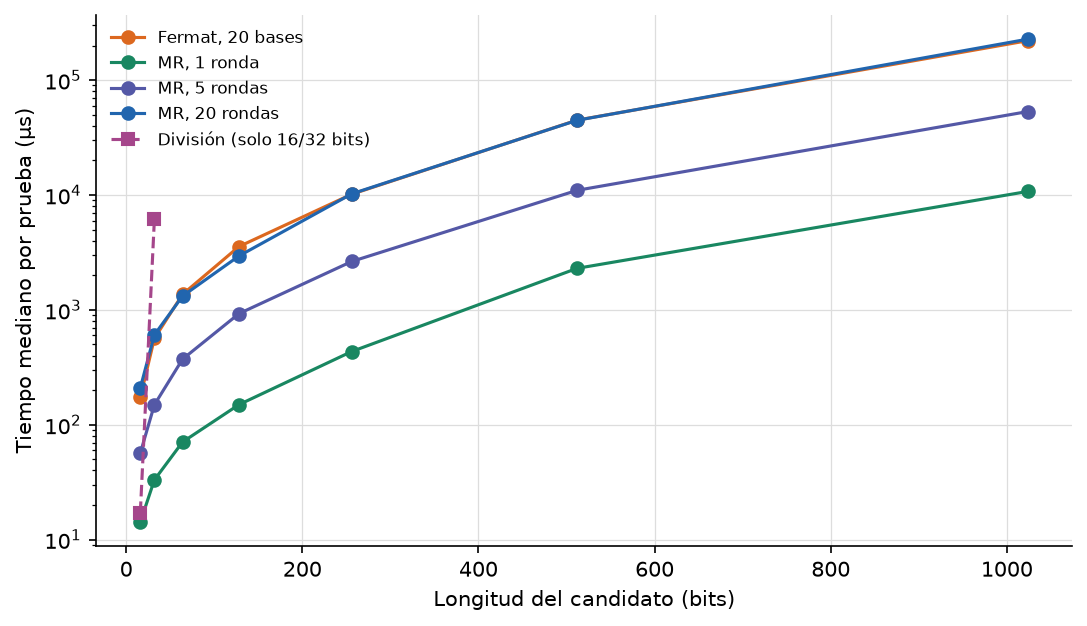
\includegraphics[width=.88\textwidth]{fig1_tiempo_vs_bits.png}
\caption{Tiempo mediano por prueba y longitud binaria; escala temporal logarítmica. La división se ejecuta solo hasta $32$ bits.}\label{fig:tiempo}
\end{figure}
\begin{figure}[H]\centering
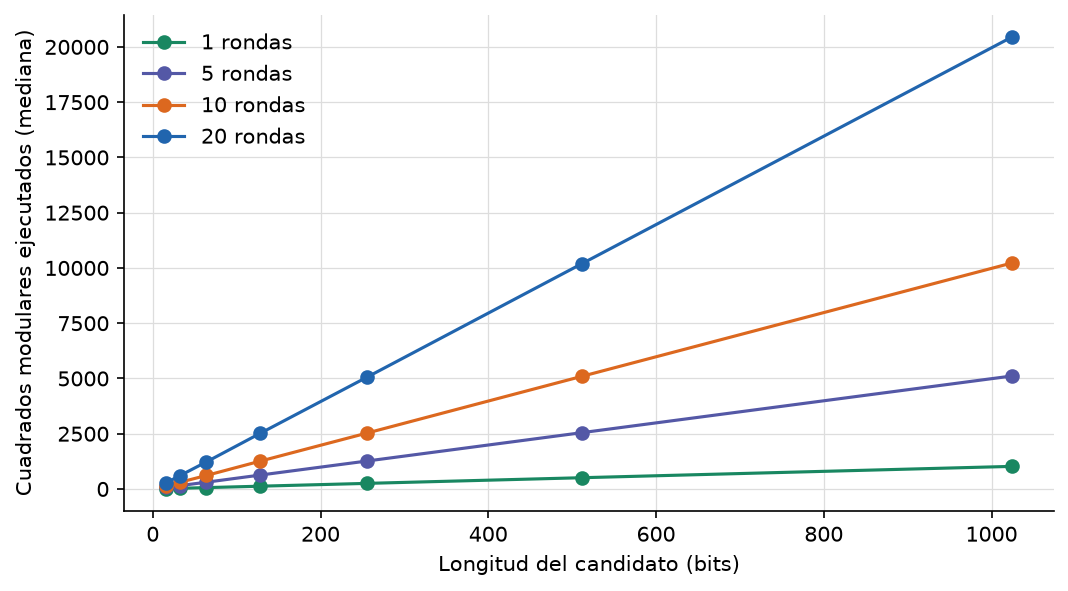
\includegraphics[width=.88\textwidth]{fig2_cuadrados_vs_bits.png}
\caption{Cuadrados modulares efectivamente realizados por Miller--Rabin con $1$, $5$, $10$ y $20$ rondas.}\label{fig:cuadrados}
\end{figure}
Las rondas terminan temprano si se encuentra un testigo de composición. Sobre candidatos aceptados se completan todas las rondas; por ello es necesario distinguir el costo de una prueba individual del costo total de buscar un probable primo.

\subsection{Generación y precribado}
El Cuadro \ref{tab:generacion} resume $30$ generaciones por tamaño: candidatos, descartes y tiempo. La semilla y los contadores individuales constan en \path{python/results/generacion_210_probables_primos.csv}.
\begin{table}[H]\centering\small
\caption{Generación de 30 probables primos por longitud binaria}
\label{tab:generacion}
\begin{tabular}{rrrrrr}\toprule
Bits & Candidatos & Media & Mediana & Descartes & Tiempo med. (ms) \\
\midrule
16 & 169 & 5.63 & 5.0 & 139 & 0.220 \\
32 & 371 & 12.37 & 10.5 & 310 & 0.720 \\
64 & 652 & 21.73 & 16.5 & 537 & 1.367 \\
128 & 970 & 32.33 & 22.5 & 806 & 3.181 \\
256 & 1840 & 61.33 & 40.5 & 1541 & 10.599 \\
512 & 5307 & 176.90 & 97.5 & 4445 & 69.182 \\
1024 & 12870 & 429.00 & 314.5 & 10833 & 802.315 \\
\bottomrule\end{tabular}\end{table}

\noindent\textbf{Lectura cuantitativa de la generación.} Para 1024 bits se necesitaron 12870 candidatos para 30 probables primos (media 429.00, mediana 314.5); el precribado descartó 10833 (84.2\%). La referencia asintótica es 354.9 candidatos impares por primo. Para 512 bits, la media observada fue 176.90 frente a 177.4 estimados. Las diferencias con la aproximación pueden reflejar variación muestral; por sí solas no prueban ni descartan errores de primalidad.\par

\begin{figure}[H]\centering
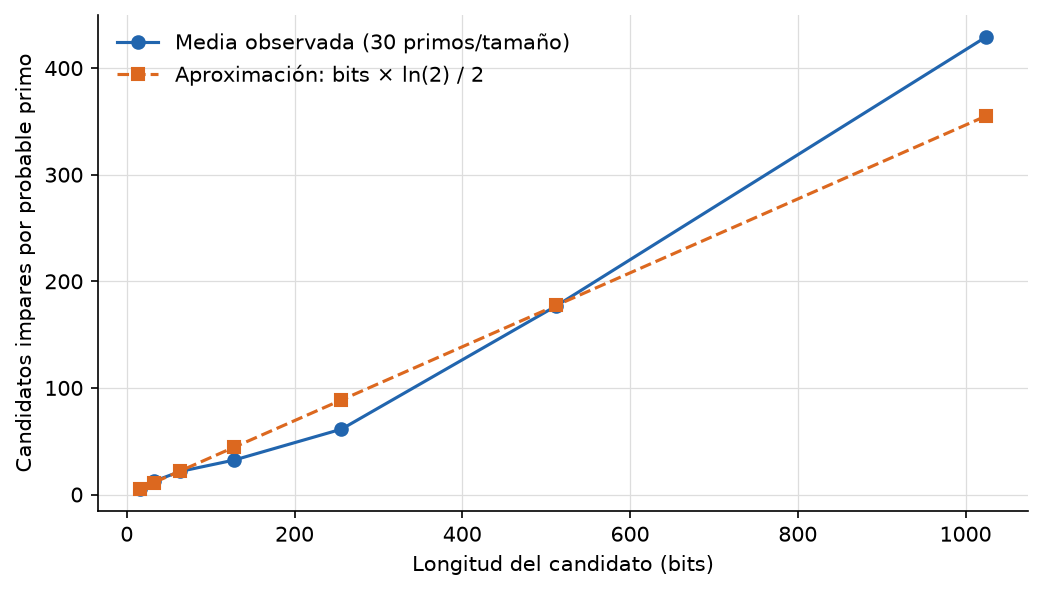
\includegraphics[width=.88\textwidth]{fig3_candidatos_vs_bits.png}
\caption{Candidatos impares por probable primo: media de $30$ muestras y aproximación $L\ln(2)/2$.}\label{fig:candidatos}
\end{figure}
El precribado evita exponenciaciones en compuestos con factores pequeños, pero no cambia la densidad de primos entre todos los candidatos originalmente muestreados.

\subsection{Testigos, mentirosos fuertes y probabilidad de error}
El Cuadro \ref{tab:mentirosos} enumera la cantidad de bases testigo y mentirosas fuertes; el archivo \texttt{clasificacion\_bases.csv} identifica cada base válida del rango pequeño. Para un compuesto impar fijo, si $p_n$ es la fracción de mentirosos fuertes, la probabilidad exacta de pasar $r$ bases elegidas uniformemente con reemplazo es $p_n^r$. La cota universal $4^{-r}$ es un límite superior, no la frecuencia esperada en una muestra concreta.
\begin{table}[H]\centering\small
\caption{Testigos y mentirosos fuertes: bases válidas de compuestos seleccionados}
\label{tab:mentirosos}
\begin{tabular}{rrrrr}\toprule
$n$ & Bases & Testigos & Mentirosos & Fracción \\
\midrule
25 & 22 & 20 & 2 & 0.0909 \\
91 & 88 & 72 & 16 & 0.1818 \\
121 & 118 & 110 & 8 & 0.0678 \\
221 & 218 & 214 & 4 & 0.0183 \\
341 & 338 & 290 & 48 & 0.1420 \\
561 & 558 & 550 & 8 & 0.0143 \\
\bottomrule\end{tabular}\end{table}

\begin{table}[H]\centering\small
\caption{Aceptación empírica y exacta de compuestos para 3000 ensayos por fila}
\label{tab:error}
\begin{tabular}{rrrrrr}\toprule
$n$ & Rondas & Aceptados & Frecuencia & Exacta $p_n^r$ & Cota $4^{-r}$ \\
\midrule
25 & 1 & 281 & 0.0937 & 0.0909 & 0.25 \\
25 & 5 & 0 & 0 & 6.21e-06 & 0.000977 \\
25 & 20 & 0 & 0 & 1.49e-21 & 9.09e-13 \\
341 & 1 & 413 & 0.138 & 0.142 & 0.25 \\
341 & 5 & 0 & 0 & 5.78e-05 & 0.000977 \\
341 & 20 & 0 & 0 & 1.11e-17 & 9.09e-13 \\
561 & 1 & 38 & 0.0127 & 0.0143 & 0.25 \\
561 & 5 & 0 & 0 & 6.06e-10 & 0.000977 \\
561 & 20 & 0 & 0 & 1.35e-37 & 9.09e-13 \\
\bottomrule\end{tabular}\end{table}

\begin{figure}[H]\centering
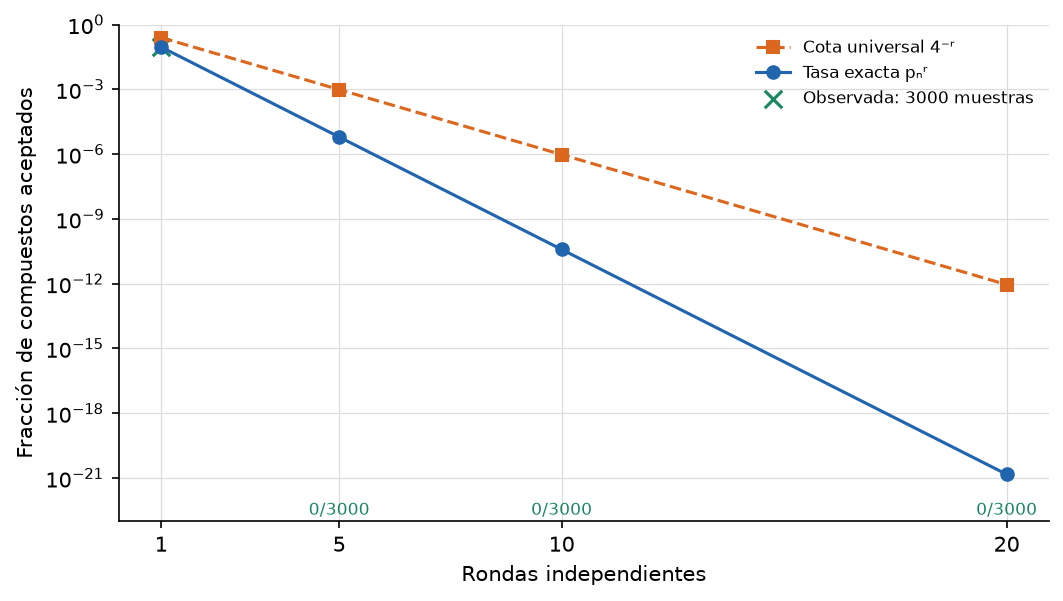
\includegraphics[width=.88\textwidth]{fig4_error_empirico.png}
\caption{Compuesto $25$: tasa exacta $p_n^r$, cota $4^{-r}$ y $3000$ ensayos por número de rondas. Los ceros observados se anotan como $0/3000$, no como probabilidades positivas.}\label{fig:error}
\end{figure}
La simulación consulta la clasificación exhaustiva de bases de $n\in\{25,91,121,341,561\}$ para $r\in\{1,5,10,20\}$; no se interpreta como una medición del tiempo de Miller--Rabin. No observar falsos positivos en una muestra finita no demuestra error nulo. Fermat no dispone de una cota análoga para números de Carmichael.


\clearpage
% Sección 5: Preguntas de análisis
% !TEX root = ../main.tex
\section{Respuestas a las preguntas de análisis}
\begin{enumerate}
\item \textbf{¿Por qué basta probar divisores hasta $\sqrt n$?} Si $n=ab$ y $a>\sqrt n$, $b>\sqrt n$, entonces $ab>n$, contradicción. Todo compuesto tiene al menos un divisor $\le\sqrt n$.

\item \textbf{¿Por qué esa cota es exponencial en bits?} Para $L$ bits, $n$ es del orden de $2^L$ y $\sqrt n$ del orden de $2^{L/2}$. Una función exponencial de $L$ no es polinómica aunque sea sublineal en $n$.

\item \textbf{¿Por qué Fermat puede demostrar composición, pero no primalidad?} Para un primo $p$ y base coprima $a$, Fermat exige $a^{p-1}\equiv1\pmod p$. Si falla, por contraposición $n$ es compuesto; si pasa, puede ser un pseudoprimo. El ejemplo $341$ con base $2$ confirma que el recíproco es falso.

\item \textbf{¿Qué diferencia hay entre pseudoprimo y número de Carmichael?} Un pseudoprimo compuesto pasa Fermat para una base específica coprima; Carmichael pasa para \emph{todas} las bases coprimas. $341$ pasa base $2$, mientras $561$ pasa cualquier base coprima. La base $3$ no es coprima a $561$ y sí lo detecta.

\item \textbf{¿Por qué Miller--Rabin examina $n-1=2^sd$?} Separar la máxima potencia de $2$ produce la cadena $a^d,a^{2d},\ldots,a^{2^{s-1}d}$. En un módulo primo, si el último término es $1$, la cadena debe comenzar en $1$ o alcanzar $-1$ antes: solo $\pm1$ son raíces de $x^2=1$ en un cuerpo.

\item \textbf{¿Qué significa encontrar una raíz no trivial de $1$?} Existe $x\not\equiv\pm1\pmod n$ con $x^2\equiv1\pmod n$. Como $(x-1)(x+1)\equiv0\pmod n$ sin que uno de esos factores sea $0\pmod n$, $n$ es compuesto. En $341$, $x=32$ y los MCD respectivos recuperan $31$ y $11$.

\item \textbf{¿Qué diferencia hay entre testigo y mentiroso fuerte?} Testigo: base cuyo resultado Miller--Rabin es negativo, prueba que el número es compuesto. Mentiroso fuerte: base cuyo resultado es positivo pese a que $n$ es compuesto. El par $(341,2)$ es testigo, aunque $2$ sea mentiroso para Fermat en $341$.

\item \textbf{¿Por qué el error es unilateral?} Toda base válida hace pasar a un número primo. El rechazo significa compuesto con certeza; la única posible equivocación es aceptar como probable primo un compuesto que superó las bases elegidas.

\item \textbf{¿Qué hipótesis permite usar $4^{-r}$?} El número evaluado debe ser compuesto impar; cada base se selecciona uniforme e independientemente entre las bases válidas. La fracción de mentirosos fuertes es $\le1/4$ y el evento de $r$ aceptaciones tiene probabilidad $\le(1/4)^r$. La semilla fija permite reproducir un experimento, no garantiza aleatoriedad criptográfica.

\item \textbf{¿Por qué una semilla fija no es apropiada para generar claves?} Permite repetir la misma secuencia de candidatos y bases. Si se conoce o adivina, un adversario reconstruye los valores generados. Se debe usar una fuente segura e impredecible como \texttt{secrets.SystemRandom}.

\item \textbf{¿Cómo influye el precribado?} Detecta compuestos divisibles por primos pequeños con divisiones baratas, evitando muchas exponenciaciones. También debe aceptar cuando el candidato coincide exactamente con uno de esos primos. Acelera la generación, pero no certifica primalidad de números grandes que lo superan.

\item \textbf{¿Por qué ``no observamos errores'' no significa ``el algoritmo no puede errar''?} Una muestra finita puede omitir las bases mentirosas. La ausencia observada no prueba probabilidad cero; hay que distinguir frecuencia empírica, probabilidad exacta $p_n^r$ para un compuesto dado y cota universal $4^{-r}$.
\end{enumerate}


% Sección 6: Conclusiones
% !TEX root = ../main.tex
\section{Conclusiones grupales}
La implementación de la Guía 07 permitió relacionar los fundamentos algebraicos con resultados verificables. La división de prueba ofrece certeza, pero su límite de aproximadamente $2^{L/2}$ divisiones para entradas de $L$ bits impide aplicarla a tamaños criptográficos. Fermat reduce el costo mediante exponenciación modular, aunque su aceptación no demuestra primalidad: $341$ supera la base $2$, y los números de Carmichael $561$, $1105$ y $1729$ superan todas las bases coprimas. Por ello, el equipo separó explícitamente los resultados ``compuesto'', ``primo certificado'' y ``probable primo''.

Miller--Rabin mostró una ventaja esencial: la cadena obtenida de $n-1=2^sd$ puede hallar testigos que Fermat no encuentra. En particular, la base $2$ rechaza a $341$ al descubrir la raíz no trivial $32$ de $1$ módulo $341$; los máximos comunes divisores con $31$ y $33$ recuperan sus factores. Las trazas registran parámetros, residuos y operaciones reales, haciendo auditables las decisiones. Comprobamos las propiedades con una suite de 32 pruebas, una criba independiente para enteros pequeños y 1000 enteros aleatorios menores que un millón contrastados con división de prueba.

Los experimentos recorren siete longitudes entre 16 y 1024 bits y producen 210 probables primos, con candidatos, descartes por precribado, rondas, cuadrados y tiempos registrados. La comparación usa las mismas entradas y bases preseleccionadas para Fermat y Miller--Rabin, evitando atribuir al azar diferencias de rendimiento. Los candidatos de 16 y 32 bits también se certificaron con división de prueba; los mayores mantienen la condición de probables primos. Medir tiempo y contar operaciones son tareas distintas: Python maneja enteros de longitud creciente y su costo no depende solo del número de rondas.

Finalmente, una tasa empírica de error nula no implica imposibilidad de error. La cota $4^{-r}$ exige bases independientes uniformes, y una semilla fija es útil para reproducibilidad, pero inapropiada para claves. Un precribado correcto ahorra exponenciaciones sin transformar por sí solo una prueba probabilística en determinista. El producto entregado conserva código, pruebas, CSV, gráficos e informe reproducibles para permitir repetir y discutir cada conclusión.


\clearpage
% Referencias bibliográficas de la guía y herramientas utilizadas
% !TEX root = ../main.tex
\begin{thebibliography}{9}
\bibitem{guia07} H. E. Ugarte Rojas, \emph{Guía de Laboratorio N.º 07: Primalidad, grupos y algoritmos probabilísticos}, Algoritmos Avanzados, UNSAAC, 2026-II.
\bibitem{cormen} T. H. Cormen, C. E. Leiserson, R. L. Rivest y C. Stein, \emph{Introduction to Algorithms}, 4.ª ed. MIT Press, 2022.
\bibitem{shoup} V. Shoup, \emph{A Computational Introduction to Number Theory and Algebra}, 2.ª ed. Cambridge University Press, 2009.
\bibitem{crandall} R. Crandall y C. Pomerance, \emph{Prime Numbers: A Computational Perspective}, 2.ª ed. Springer, 2005.
\bibitem{pythonsecrets} Python Software Foundation, \emph{secrets --- Generate secure random numbers}. \url{https://docs.python.org/3/library/secrets.html}.
\end{thebibliography}


\end{document}
